
\chapter{Erstes Kapitel}
\label{sec:first}

Ein Kapitel.

\begin{figure}[htb] %  figure placement: here, top, bottom
\centering

\includegraphics{Images/Chapter/trouble}
\caption{Trouble \ldots}
\label{fig:trouble}
\end{figure}

\blindtext\blindtext

\blindtext


\chapter{Zweites Kapitel}
Um das vorherige Kapitel zu lesen, siehe Kapitel \ref{sec:first}.


\section{Zweite Gliederugsebene...}

Es darf nun weiterer gewichtiger Inhalt folgen.
Hier werden nun einige grundlegenden \LaTeX-Kommandos demonstriert.

\subsection{Dritte Gliederungsebene}

Man kann aber noch tiefer Gliedern

\subsubsection{Vierte Gliederungsebene}

Drei Gliederungsebenen sollten für kleine Artikel und Ausarbeitungen genügen. 
Anderenfalls sollte die Strukturierung nocheinmal überdacht werden.

\paragraph{Paragraph ist die unterste Ebene} \blindtext

\section{Tabellen einbinden}

\begin{table}
\centering
\begin{tabular}{|c||lr|}\hline
1.1 & 1.2 & 1.3 \\ \hline
2.1 & 2.2 & 2.3 \\ \hline \hline
3.1 & 3.2 & 3.3 \\ \hline
\end{tabular}
\caption{Eine simple Tabelle}\label{tab:simple}
\end{table}


Tabellen sollten in einer Table-Umgebung eingefügt und mit einer Caption und einem Label versehen werden.
Ein einfaches Beispiel zeigt Tabelle \ref{tab:simple}.

Leider sind Tabellen eines der schwierigeren Kapitel in \LaTeX,
wenn beispielsweise Zellen zusammengefasst werden.
Tabelle \ref{tab::komplex} zeigt eine etwas aufwendigere Tabelle.


\begin{table}
\centering
\begin{tabular}{c|c|c|c|c|}	
	\multicolumn{2}{c}{}
	& \multicolumn{3}{c}{\begin{scriptsize}\textbf{GdO-Typ}\end{scriptsize}}
	\\ \hhline{~~---}
	\multicolumn{2}{c|}{}
	& \textbf{reellwertig}
	& \textbf{ganzzahlig}
	& \textbf{symbolisch}
	\\ \hhline{~|----}
	\multirow{4}[3]{*}{\rotatebox{90}{\begin{scriptsize}\textbf{EA-Typ}\end{scriptsize}}}
	& \textbf{reellwertig}
	& direkt
	& Rundung
	& ---
	\\ \hhline{~|----}
	& \textbf{ganzzahlig}
	& ---
	& direkt
	& Index
	\\ \hhline{~|----}
	& \textbf{Zeichenkette}
	& Interpretation
	& Interpretation
	& direkt
	\\ \hhline{~|----}
\end{tabular}
\caption{Beispiel für eine komplexere Tabelle}\label{tab::komplex}
\end{table}

\section{Bilder/Grafiken einbinden}

Am besten werden Vektorgrafiken verwendet.
Diese liegen im Idealfall als PDF vor.
Aber auch EPS kann z.B. sehr einfach konvertiert werden.

PDF-Grafiken können unter anderem mit Inkscape \cite{inkscape}, OpenOffice Draw \cite{oodraw} kostenlos bearbeitet und erstellt werden.
Pixelgrafiken sollten unbedingt vermieden werden. 
Ihre Auflösung sollte mind. 300dpi betragen.

\subsection{Einfache Abbildungen}

\begin{figure}
\centering % zentriert alles in der Figure
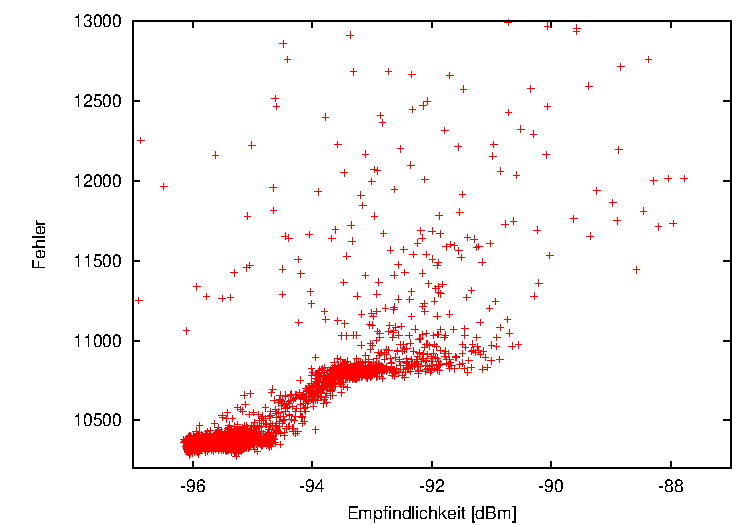
\includegraphics[width=0.6\linewidth]{Images/Chapter/bspgrafik1} % externe Grafik laden
\caption{Dieses Diagramm ist ein Beispiel für eine einfache Abbildung.}\label{fig:testabb}
\end{figure}


Eine Abbildung sollte sich immer in einer Figure-Umgebung befinden.
In dieser kann sie mit einer Caption beschrieben werden
und sie kann über ein Label gekennzeichnet werden (vgl. Abbildung \ref{fig:testabb}).

Dabei muss es keine Grafik sein, die in eine Figure-Umgebung geladen wird.
Es kann dort ganz normal \LaTeX geschrieben werden,
wie Abbildung \ref{fig:testabb2} zeigt.

\begin{figure}
\centering
\fbox{\parbox{0.9\linewidth}{\centering In einer Figure muss keine Grafik stehen... Eine Abbildung kann im Prinzip alles sein.}}
\caption{Dies ist eine Bildunterschrift} \label{fig:testabb2}
\end{figure}

\subsection{Unterabbildungen}

\begin{figure}%
  \centering
   \subfloat[Die erste Unterabbildung]{\label{fig:subfig1}%
       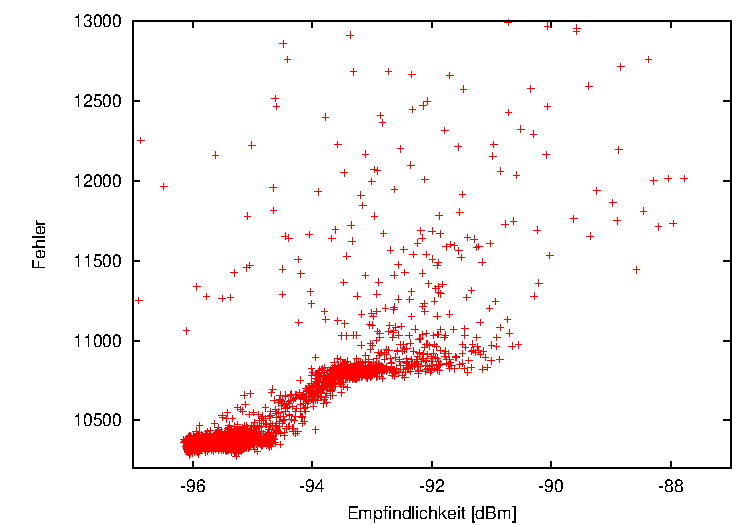
\includegraphics[width=0.48\linewidth]{Images/Chapter/bspgrafik1}
   }\hfill
   \subfloat[Die zweite Unterabbildung]{\label{fig:subfig2}%
       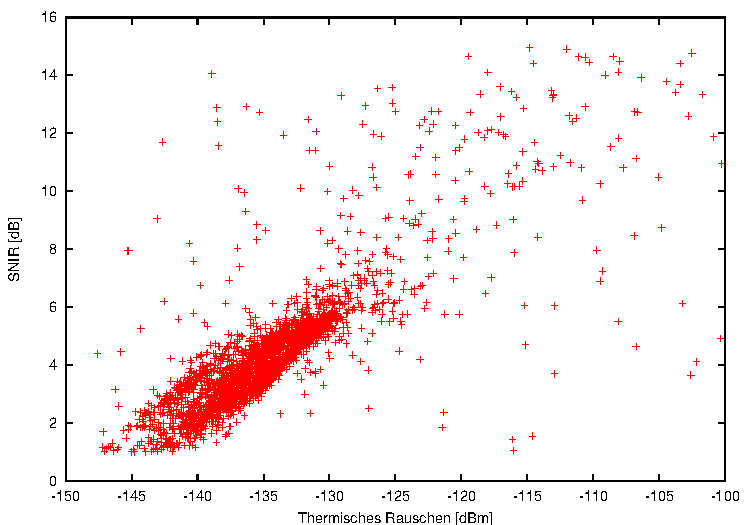
\includegraphics[width=0.48\linewidth]{Images/Chapter/bspgrafik2}
   }
   \caption{Beispiel für Unterabbildungen}
   \label{fig:subfigexample}
\end{figure}


In manchen Fällen ist es sinnvoll eine Abbildung in Unterabbildungen zu teilen.
In Abbildung \ref{fig:subfigexample} wird dies gezeigt.
Die Abbildungen \ref{fig:subfig1} und \ref{fig:subfig2} sind Unterabbildungen.

\section{Formeln}

Für seinen Formelsatz ist \LaTeX besonders bekannt, weshalb es hier nicht an einem kleinen Beispiel (vgl. Formel \ref{eq::gewichtsumme}) fehlen soll.

\begin{equation}
f\idx{sim}(g,U)=\sum\limits^{n\idx{M}}_{\mu=1} w_\mu\cdot c_i( M_\mu(g,U)) \label{eq::gewichtsumme}
\end{equation}

\section{Quelltexte einbinden}

\begin{figure}[t]
\begin{lstlisting}[language=java, caption={Beispiel für ein Listing},  label=lst:bsplst]
public class RadioFitness extends BasicFitness {
  ...
  SimResultReader result = new SimResultReader();
  ...
  protected void readResult(Scenario s) throws FitnessException {
    result.readFrom(s.getExecEnv().getExecutionDir());
  }

  protected double getRawMetric(String name) throws FitnessException {
    if(name.equals("delivery rate")
      return result.getNumSendData()/result.getNumReceivedData();
    else if(name.equals("latency"))
      return results.getLatency();
    else ...
  } // comment
  ...
}
\end{lstlisting}
\end{figure}


Ein Beispiel für ein Java-Listing zeigt Listing \ref{lst:bsplst}.


\section{Zitieren von Quellen}

Aussagen wollen gut belegt sein.
Hier sind willkürlich \cite{FejF08} beispielhafte Zitierungen \cite{Deming1986} angegeben,
die keinen inhaltlichen Bezug zu diesem Text aufweisen.
Vielmehr geht es darum beispielhaft zu zitieren.
Es können auch mehrere Quellen angegeben werden \cite{biturl,Rost2009} (auch hier wieder ohne inhaltlichen Bezug).

Die Literaturangaben werden in einer Datenbank verwaltet,
die in einer .bib-Datei gespeichert wird.
In dieser kann auch nicht zitierte Literatur stehen.
Eine gute Software zur Bearbeitung dieser Datenbank ist JabRef \cite{jabref}.